%% LyX 2.0.4 created this file.  For more info, see http://www.lyx.org/.
%% Do not edit unless you really know what you are doing.
\documentclass[12pt,UTF8, adobefonts]{ctexart}
\usepackage[T1]{fontenc}
\pagestyle{plain}
\usepackage{graphicx}
\usepackage{setspace}
\onehalfspacing

\makeatletter
%%%%%%%%%%%%%%%%%%%%%%%%%%%%%% Textclass specific LaTeX commands.
\newenvironment{lyxcode}
{\par\begin{list}{}{
\setlength{\rightmargin}{\leftmargin}
\setlength{\listparindent}{0pt}% needed for AMS classes
\raggedright
\setlength{\itemsep}{0pt}
\setlength{\parsep}{0pt}
\normalfont\ttfamily}%
 \item[]}
{\end{list}}

%%%%%%%%%%%%%%%%%%%%%%%%%%%%%% User specified LaTeX commands.
% 如果没有这一句命令,XeTeX会出错,原因参见
% http://bbs.ctex.org/viewthread.php?tid=60547
\DeclareRobustCommand\nobreakspace{\leavevmode\nobreak\ }
\date{}

\makeatother

\begin{document}

\title{FPGA-based Solution for Reverse Time Migration 中文介绍}


\author{作者:何聪辉\\
指导老师:陈立文}

\maketitle

\section{简介}

地质勘探的目的是为了挖掘地球内部的矿产资源,如石油,天然气。比如,如果要勘探海底的地址结构,轮船可以通过空气炮的形式向海底发射声波,同时在多个地方收集海底不同介质反射回来的地震波,对收集到的地震波进行处理,逆向生成海底的地质结构,从而判断是否有矿产资源的存在。过去使用的算法,比如Ray
Trace, 适用于较为简单的地质结构,如水层下面是盐层,盐层下面是岩石层,层的形状基本上为水平状,不存在大幅度的倾角;但面对较为复杂的地址结构,如盐层的倾角大于70度,层间复杂交错,传统的算法无法准确对此结构进行成像。
\begin{figure}
\begin{centering}
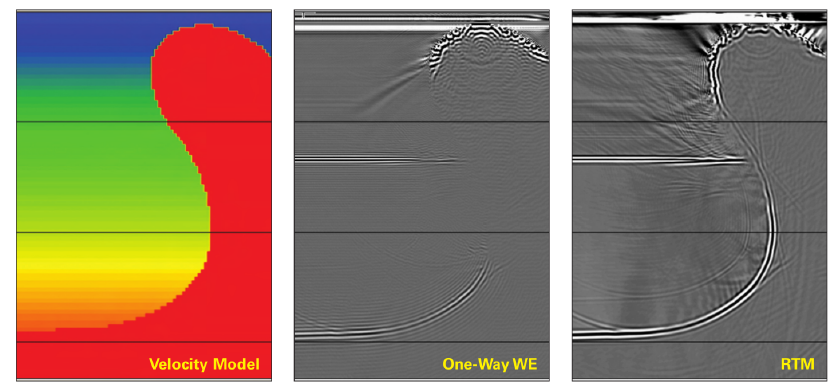
\includegraphics[scale=0.6]{rtm}
\par\end{centering}

\caption{RTM算法与单向便宜算法的比较\label{fig:RTM=007B97=006CD5=004E0E=005355=005411=004FBF=005B9C=007B97=006CD5=007684=006BD4=008F83}}


\end{figure}


正如图(\ref{fig:RTM=007B97=006CD5=004E0E=005355=005411=004FBF=005B9C=007B97=006CD5=007684=006BD4=008F83})所示,单向的声波方程在边界较为陡峭的地方无法准确成像,这很有可能忽略了存在的矿产资源。偏移(Reverse
Time Migration)算法能够对复杂的地质结构进行较为准确的成像,但是该算法的计算量非常大,CPU版本的算法复杂度约为O(n\textasciicircum{}3),且伴随着非常大的常数,再加上需要处理的数据量非常大,通常是TB数量级,该算法在工业界的使用尚不广泛。但目前随着计算机计算力的提升以及加速卡,如GPU,FPGA,的出现,为加速该算法提供了很大的可能性。本文利用FPGA作为加速器,在FPGA上实现该算法,目前的版本相对8核的Intel
i7的CPU而言,得到了6倍的加速效果,且具有很大的优化空间。

Field Programming Gate Array (FPGA) 是一个可编程的硬件。通过对FPGA进行算法设计,代码直接通过硬件执行,而非通过操作系统的调度,因此具有非常高的效率。但在FPGA上设计算法是一件非常难的事情,传统的方法是通过硬件描述语言(HDL)对其进行编程,开发者需要关注每一个电路逻辑单元,这也是为什么FPGA较CPU,
GPU或其他嵌入式设备而言,并没有那么流行的原因。本文利用Xilinx公司的FPGA芯片,Maxeler公司的MaxCompiler,在一个稍高的抽象层对FPGA进行设计,实现RTM算法。


\section{研究内容}


\subsection{基于声波的正演(Forward Modeling)}

Reverse Time Migration 算法的核心是正演(forward modeling)。当地震波(声波)从波源发出后,从中心(波源)想四周扩散,当遇到边界(如盐层和岩石层之间的边界)时,同时进行反射和折射,以及部分能量被吸收。正演正是模拟这个过程。在计算机处理过程中,以一个网格划分的三维数组存储特定空间的波场
(wave field) ,正演的操作则是根据$t$和$t-1$时刻的波场,得出$t+1$时刻的波场。设$u$ 为当前时刻的波场,$c$为当前正演的速度模型(声波在特定区域的速度),
$s$为当前时刻波源的能量,则正演使用的声波方程为

\begin{eqnarray}
F=\frac{\partial^{2}u}{\partial t^{2}} & = & c^{2}\cdot(\bigtriangledown^{2})u+s\label{eq:1}
\end{eqnarray}


其中,$\bigtriangledown$为Laplace算子,如果用二阶偏微分方程将其近似,可以得到如下的式子(\ref{eq:2})

\begin{eqnarray}
\bigtriangleup u & = & \bigtriangledown^{2}u=\frac{\partial^{2}u}{\partial x^{2}}+\frac{\partial^{2}u}{\partial y^{2}}+\frac{\partial^{2}u}{\partial x^{2}}\label{eq:2}
\end{eqnarray}


将Laplace的近似代入(\ref{eq:1}),同时将$\frac{\partial^{2}u}{\partial t^{2}}$离散化,可以得到式子(\ref{eq:3})

\begin{eqnarray}
\frac{u_{t+1}-2u_{t}+u_{t-1}}{dt^{2}} & = & c_{t}^{2}\cdot(\frac{\partial^{2}u_{t}}{\partial x^{2}}+\frac{\partial^{2}u_{t}}{\partial y^{2}}+\frac{\partial^{2}u_{t}}{\partial x^{2}})+s_{t}\label{eq:3}
\end{eqnarray}


在计算中,连续的偏微分方程可以通过有限差分的方法转换为差分方程,如此便可在计算网格中算出每个点的值。本文使用stencil方法对$\frac{\partial^{2}u_{t}}{\partial x^{2}}+\frac{\partial^{2}u_{t}}{\partial y^{2}}+\frac{\partial^{2}u_{t}}{\partial x^{2}}$在$u(t,x,y,z)$进行求值。若采用6阶的stencil,stencil在点$(x,y,z)$的值为

\begin{eqnarray*}
g(x,y,z) & = & \sum_{i=-3}^{+3}w_{i}f(i,y,z)+\sum_{i=-3}^{+3}w_{i}f(x,i,z)+\sum_{i=-3}^{+3}w_{i}f(x,y,i)-2f(x,y,z)
\end{eqnarray*}


图(\ref{fig:6=009636=004E09=007EF4stencil})勾画了6阶的三维stencil操作所要用到的点。
\begin{figure}
\begin{centering}
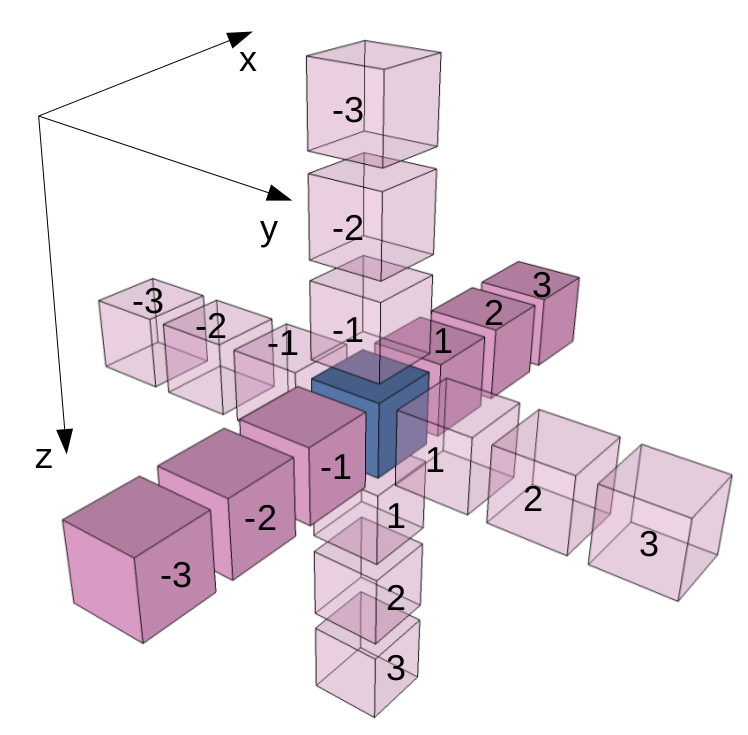
\includegraphics[scale=0.4]{stencil}
\par\end{centering}

\caption{6阶三维stencil所涉及到的点\label{fig:6=009636=004E09=007EF4stencil}}
\end{figure}


设研究的整个波场为$x\times y\times z$的数组,则在每一次的迭代中,需要对$x\cdot y\cdot z$个点进行stencil操作,在实际应用中,$x\approx y\approx z\approx10^{4}$,迭代次数$t\approx10^{4}$,因此对于一次的波源冲击,需要进行$10^{16}$浮点运算,这通常在CPU上是无法忍受的。况且现实生活中,往往有多次波源冲击以获得更加准确的数据。图(\ref{fig:=0057FA=004E8E=0058F0=006CE2=0065B9=007A0B=007684=006B63=006F14=007B97=006CD5=007684=004F2A=004EE3=007801})是基于声波方程的正演算法的伪代码,通过嵌套的循环数量可以推测该算法惊人的复杂度。
\begin{figure}
\begin{centering}
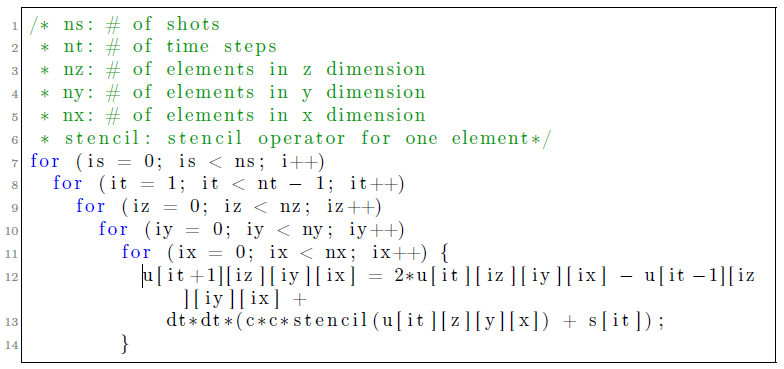
\includegraphics[scale=0.65]{acoustic}
\par\end{centering}

\caption{基于声波方程的正演算法的伪代码\label{fig:=0057FA=004E8E=0058F0=006CE2=0065B9=007A0B=007684=006B63=006F14=007B97=006CD5=007684=004F2A=004EE3=007801}}


\end{figure}



\subsection{基于声波的逆时偏移 (Revese Time Migration)}

令从波源开始的正演方程为为$F_{t=t_{0}}^{t_{n}}$,代表着从$t_{0}$时刻开始正演,直到$t_{n}$时刻结束。对每个接收点接收到的数据进行逆向正演$F_{t=t_{n}}^{t_{0}}$,代表着从$t_{n}$时刻开始正演,逐步后退,直到$t_{0}$时刻停止。而Reverse
Time Migration则取每个点的正向正演和逆向正演的乘积作为改点的成像值。图(\ref{fig:=0057FA=004E8E=0058F0=006CE2=0065B9=007A0B=007684RTM=007B97=006CD5=004F2A=004EE3=007801})是基于声波方程的RTM算法的伪代码。对于网格中的每个点,需要进行两次正演,可见RTM算法的计算量约为单次正演计算量的两倍。
\begin{figure}
\begin{centering}
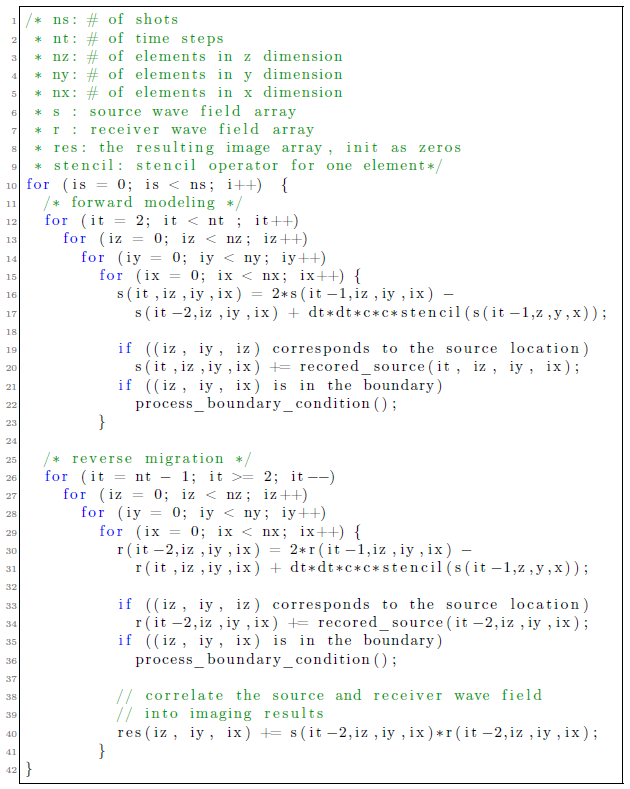
\includegraphics[scale=0.9]{rtm_code}
\par\end{centering}

\caption{基于声波方程的RTM算法伪代码\label{fig:=0057FA=004E8E=0058F0=006CE2=0065B9=007A0B=007684RTM=007B97=006CD5=004F2A=004EE3=007801}}


\end{figure}


本文正是完成该算法在FPGA上的实现,以求获得比当前CPU实现更高的效率。


\section{研究方法}

本文的重心在于RTM算法在FPGA上的设计与实现,因此,省略了介绍如何搭建FPGA开发环境,如何调试及测试,尽管这是一个工作量大,学习曲线陡峭的过程。


\subsection{FPGA编程范式}

FPGA的编程范式是高级语言(C/C++)开发者难以适应的。FPGA展现在开发者(设计者)面前的是许多资源,如加法器,选择器,计数器,锁存器等等。开发者需要根据自己的需要,思考如何连接不通的器件,使其能够按照开发者的意图工作。这通常通过硬件描述语言(HDL)完成。个别厂商,如Maxeler,为了方便一般程序员重新学习硬件描述语言,使用了Java语言对底层的元器件和功能进行封装并提供接口,因此,开发者可以通过购买Maxeler提供的开发工具,使用Java进行开发。但Java只是作为一种描述的语言,整个FPGA开发的范式与思想与传统的利用操作系统调度的程序截然不同。

FPGA的设计不存在一般编程中的循环(while),分支(if/else)等控制指令,而是以流的形式完成计算的。这个因为FPGA中并不存在像CPU这样的处理器,能够完成复杂的跳转操作,只有许多简单的元器件,元器件一旦连接完成,在每个时钟周期,每个输入既能产生对应的输出。因此,本文的难点也在于如何将图(\ref{fig:=0057FA=004E8E=0058F0=006CE2=0065B9=007A0B=007684RTM=007B97=006CD5=004F2A=004EE3=007801})伪代码中复杂的循环(for)和分支(if/else)以及数组元素访问指令通过简单的FPGA元器件完成。


\subsection{数组元素访问}

FPGA中有许多元器件,也包括DRAM,但是没有抽象意义上的数组,自然不存在所谓的数组元素访问。但绝大多数的问题都是需要通过数组完成的,如何在FPGA上完成数组的访问是迫切需要解决的问题。

由于FPGA的电路设计完成后,在每个时钟周期,一个输入对应一个输出,当前时钟周期能够访问的数组元素就是当前的输入。如果没有对当前的输入进行存储,下一个时钟周期的输入将覆盖当前的输入,因此当前的输入在以后的时钟周期中无法再次访问。针对RTM算法,如图(\ref{fig:=0057FA=004E8E=0058F0=006CE2=0065B9=007A0B=007684=006B63=006F14=007B97=006CD5=007684=004F2A=004EE3=007801})所示,每个时钟周期需要访问过去的三个数组元素(u{[}i-3{]},
u{[}i-2{]}, u{[}i-1{]})和未来的三个元素(u{[}i+1{]}, u{[}i+2{]}, u{[}i+3{]}),这可以通过FPGA中的stream
offset完成。

stream window由锁存器组成,在当前时钟周期,stream window储存着过去三个时钟周期的输入,同时取得未来三个时钟周期的输入。
\begin{figure}
\begin{centering}
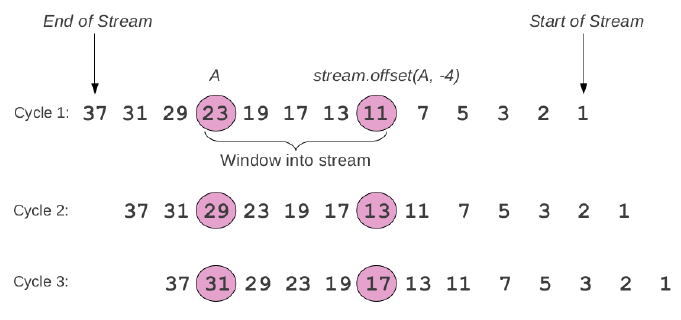
\includegraphics[scale=0.6]{stream_offset}
\par\end{centering}

\caption{3个时钟周期的stream offset 示例\label{fig:3=004E2A=0065F6=00949F=005468=00671F=007684stream-offset-=00793A=004F8B}}


\end{figure}
图(\ref{fig:3=004E2A=0065F6=00949F=005468=00671F=007684stream-offset-=00793A=004F8B})显示了三个时钟周期里,stream
window的变化情况。图(\ref{fig:3=004E2A=0065F6=00949F=005468=00671F=007684stream-offset-=00793A=004F8B})中,stream中的第一个元素为1,最后一个元素为37,当前元素为23,stream
window中储存着过去的4个元素,则可以通过stream offset的形式访问数组元素u{[}i-4{]}。当进入下一个时钟周期时,stream
window以循环队列的形式,将队首的元素(11),弹出队列,同时压入最新的元素(29)。如此方式即可访问数组中的非自身元素。

该方法并不适应与所有数组元素的访问,适用于本算法是因为RTM算法的数组元素访问存在一定的规律性,该方法能够有效利用FPGA资源高效在一个时钟周期内完成元素的访问。


\subsection{模拟循环(for)操作}

如果面对的不是一维数组,而是二维或者三维数组,访问的元素就没有很强的规律性,如当前元素的前3个。RTM算法中,每次需要判断该元素是否是边界元素,因此涉及到该元素的坐标$(x,y,z)$。其中一种方法是将三维数组铺平,变成一维数组,但是计算点$(x,y,z)$在一维数组中对应的坐标。显然,对于三维数组,这种计算极为复杂,例如,若$(3,3,3)<(x,y,z)<(nx-3,ny-3,nz-3)$代表该元素为非边界元素,将其展开围一维数组,则无法利用少量的判断条件来判断改点是不是边界点。因此,思考如何利用FPGA硬件来直接模拟循环是个不错的想法。

循环是高级语言编程中常见的控制操作,绝大多数的算法都需要循环来完成迭代和控制。但是FPGA中并不存在如此复杂的控制,如何通过元器件之间的组织和衔接来灵活模拟高级语言中的循环操作是本文实现的难点之一。

本文采用多个计数器(counter)共同协作的方式模拟循环操作。对于RTM算法的3维 stencil操作,需要控制x,y,z三个维度的变量,则需要三个计数器来完成。例如,若需要完成如下嵌套循环操作

\begin{center}
\begin{minipage}[t]{1\columnwidth}%
\begin{lyxcode}
for~(z~=~0;~z~<~nz;~z++)~\{

~~for~(y~=~0;~y~<~ny;~y++)~\{

~~~~for~(x~=~0;~x~<~nx;~x++)~\{

~~~~~~//~operations~here

~~~~\}

~~\}

\}\end{lyxcode}
%
\end{minipage}
\par\end{center}

则可以通过以下步骤完成。
\begin{enumerate}
\item 使用第一个计数器counterX,用以模拟循环中x的行为。这个计数器的特征较为简单,计数器从0开始计数,每个时钟周期,计数器的值递增1,当到达nx-1时,计数器重新返回0(该操作成为wrap)重新计数。该设计中,需要按照上述的特征描述计数器对应的参数。
\item 使用第二个计数器counterY,该计数器具有与counterX类似的特征,唯一不同的是,counterY并不是每个时钟周期递增1,而是每经过nx个时钟周期递增1。然而,FPGA中的计数器总是会在下一个时钟周期到来时递增。因此采用额外的方式对其进行控制。对于每一个元器件,都可以设置其是否激活(enable),enable状态的元器件会正常工作,而disable状态的元器件的不工作。在设计counterY时,将counterX与counterY级联(cascade),并将counterX的wrap输出脉冲连接到counterY的enable引脚。如此,则当counterX到达最大值,重新返回0(wrap)时,wrap输出的高电平电压能够是counterY处于enable状态,counterY计数器递增1。
\item 第三个计数器counterZ的设计方法与counterY的设计方式相同,将counterY与counterZ级联,并将counterY的wrap输出脉冲连接到counterZ的enable引脚。
\end{enumerate}
上述的利用计数器的方法可以较为灵活的模拟循环操作。


\subsection{模拟分支、逻辑与(\&\&)、逻辑或(||)操作}

RTM算法需要判断每个点是否为边界点,这需要复杂的分支和逻辑与判断操作,但是这些在FPGA中并不存在,只有通过元器件的方式模拟该操作。

简单的两路逻辑操作可以直接通过现成的multiplexer元器件完成,但面对复杂的判断操作,如
\begin{lyxcode}
if~(x~>=~3~\&\&~x~<~nx~-~3)
\end{lyxcode}
则无法通过一个multiplexer完成,因为每个multiplexer只有一个select input,而FPGA中并不提供逻辑与(\&\&)和逻辑或(||)操作%
\footnote{这两种操作在元器件的实现上必须存在短路,这在FPGA的流处理设计中是不现实的%
},只有位与(\&)和位或(|)。本文提出的方法是通过位与(\&)和位或(|)来替代逻辑与(\&\&)和逻辑或(||)操作。

将x >= 3的输出与 x < nx-3的输出作为位与(\&)的输入,同时将位与(\&)的输出作为multiplexer的select
input,则可以模拟上述的分支操作。


\subsection{外部控制}

由于并不是所有的CPU操作都能转换成FPGA操作,且根据FPGA的流处理特性,本文只将计算量最大的地方移到FPGA中进行计算。其他的控制,如控制RTM算法中的时间步,控制冲击波的次数,等外部循环将交由CPU控制。这当然存在优化的空间,可以是算法进一步得到加速。


\section{研究结果与展望}

通过将计算最密集的部分移植到Xilinx FPGA上,针对较小规模的数据进行实验验证和分析,然后运行时间与8核的Intel i7处理器相比,得到了6倍的性能提升。表(\ref{fig:FPGA=004E0ECPU=007684=005E73=0053F0=007279=005F81})描述了两种实现的平台特性。
\begin{table}
\begin{centering}
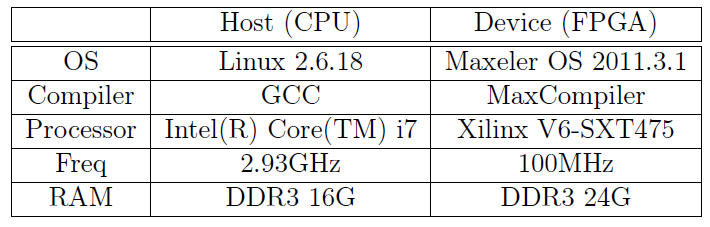
\includegraphics[scale=0.7]{comparison}
\par\end{centering}

\caption{FPGA与CPU的平台特征\label{fig:FPGA=004E0ECPU=007684=005E73=0053F0=007279=005F81}}


\end{table}
与CPU相比,FPGA的主频非常低,这也决定了FPGA相对CPU而言具有非常低的功耗,这对于大规模的集群而言,具有深刻的意义,因为CPU的高主频将为公司带来巨额电费开销。

由于当前机器的局限性和为了考虑实验的效率,本文并未采用大规模的数据进行测试,当time steps (迭代次数)为10时,波场传播空间的规模从$16\times16\times16$到$416\times416\times416$进行测试,将所耗费的时间(秒)画成曲线,得到如图(\ref{fig:=006BD4=008F83=005F53size=0053D8=005316=0065F6=00FF0CCPU=00548CFPGA=006240=0082B1=008D39=007684=0065F6=0095F4})所示的结果。
\begin{figure}
\begin{centering}
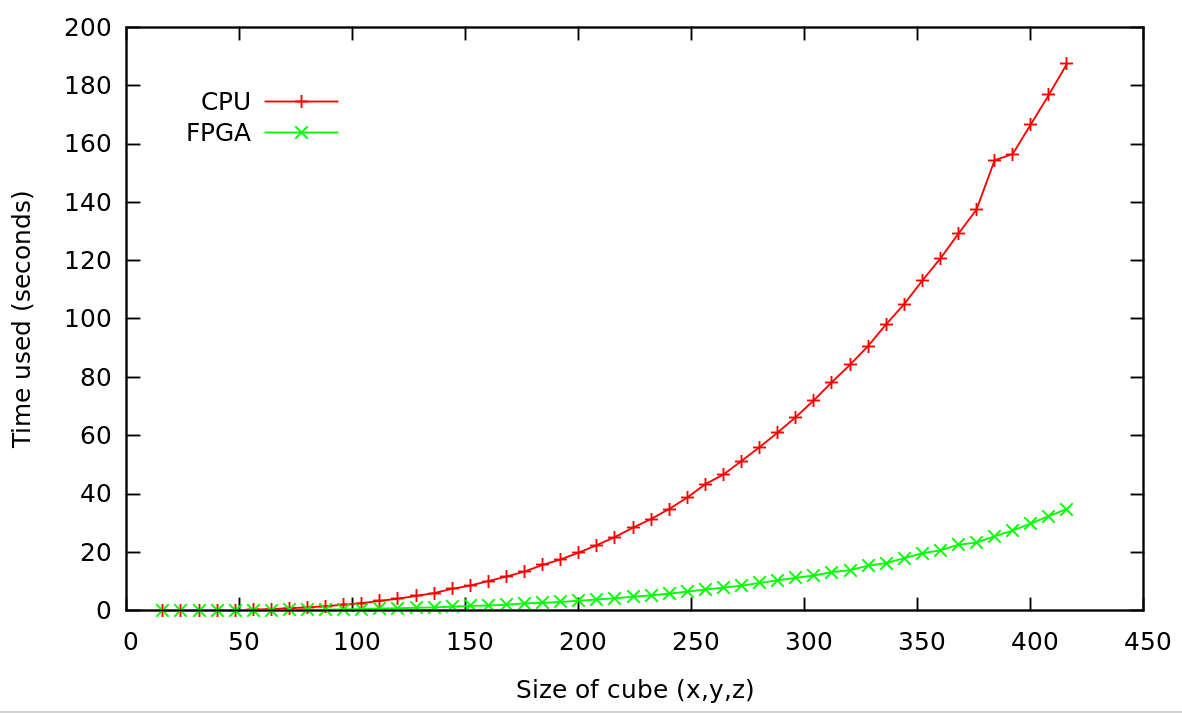
\includegraphics[scale=0.35]{result}
\par\end{centering}

\caption{\label{fig:=006BD4=008F83=005F53size=0053D8=005316=0065F6=00FF0CCPU=00548CFPGA=006240=0082B1=008D39=007684=0065F6=0095F4}比较当size变化时,CPU和FPGA所花费的时间}


\end{figure}


从(\ref{fig:=006BD4=008F83=005F53size=0053D8=005316=0065F6=00FF0CCPU=00548CFPGA=006240=0082B1=008D39=007684=0065F6=0095F4})可以看出,随着规模的增大,CPU所花费的时间迅速增长,实际上,stencil算法的复杂度为$O(n^{3})$,CPU曲线也会以$O(n^{3})$的速度增长,这在大数据量面前是难以忍受的。

相对CPU而言,FPGA的实现方案优势较为明显,曲线增长的速率较CPU而言明显降低。目前尚未能准确分析FPGA实现的复杂度。

该FPGA实现并未经过任何优化,优化FPGA的实现需要对FPGA进行更加深入的认识,包括设计的技巧,资源的选择和利用等等。因此,本文的下一步工作则是针对RTM算法,在FPGA上逐步进行优化,已获得更高的效率。
\end{document}
